%% shallow_perf.tex
%%
% Also note that the "draftcls" or "draftclsnofoot", not "draft", option
% should be used if it is desired that the figures are to be displayed in
% draft mode.
%
\documentclass[journal]{IEEEtran}
%
% If IEEEtran.cls has not been installed into the LaTeX system files,
% manually specify the path to it like:
% \documentclass[journal]{../sty/IEEEtran}

% Also, note that IEEEtran.cls V1.7 and later provides a builtin
% \ifCLASSINFOpdf conditional that works the same way.
% When switching from latex to pdflatex and vice-versa, the compiler may
% have to be run twice to clear warning/error messages.

\usepackage{cite}

% *** GRAPHICS RELATED PACKAGES ***
%
\ifCLASSINFOpdf
  \usepackage[pdftex]{graphicx}
  % declare the path(s) where your graphic files are
  % \graphicspath{{../pdf/}{../jpeg/}}
  % and their extensions so you won't have to specify these with
  % every instance of \includegraphics
  \DeclareGraphicsExtensions{.pdf,.jpeg,.png}
\else
  % or other class option (dvipsone, dvipdf, if not using dvips). graphicx
  % will default to the driver specified in the system graphics.cfg if no
  % driver is specified.
  \usepackage[dvips]{graphicx}
  % declare the path(s) where your graphic files are
  % \graphicspath{{../eps/}}
  % and their extensions so you won't have to specify these with
  % every instance of \includegraphics
  \DeclareGraphicsExtensions{.eps}
\fi


% *** MATH PACKAGES ***
%
%\usepackage[cmex10]{amsmath}
% A popular package from the American Mathematical Society that provides
% many useful and powerful commands for dealing with mathematics. If using
% it, be sure to load this package with the cmex10 option to ensure that
% only type 1 fonts will utilized at all point sizes. Without this option,
% it is possible that some math symbols, particularly those within
% footnotes, will be rendered in bitmap form which will result in a
% document that can not be IEEE Xplore compliant!
%
% Also, note that the amsmath package sets \interdisplaylinepenalty to 10000
% thus preventing page breaks from occurring within multiline equations. Use:
%\interdisplaylinepenalty=2500
% after loading amsmath to restore such page breaks as IEEEtran.cls normally
% does. amsmath.sty is already installed on most LaTeX systems. The latest
% version and documentation can be obtained at:
% http://www.ctan.org/tex-archive/macros/latex/required/amslatex/math/

% *** SPECIALIZED LIST PACKAGES ***
%
%\usepackage{algorithmic}
% algorithmic.sty was written by Peter Williams and Rogerio Brito.
% This package provides an algorithmic environment fo describing algorithms.
% You can use the algorithmic environment in-text or within a figure
% environment to provide for a floating algorithm. Do NOT use the algorithm
% floating environment provided by algorithm.sty (by the same authors) or
% algorithm2e.sty (by Christophe Fiorio) as IEEE does not use dedicated
% algorithm float types and packages that provide these will not provide
% correct IEEE style captions. The latest version and documentation of
% algorithmic.sty can be obtained at:
% http://www.ctan.org/tex-archive/macros/latex/contrib/algorithms/
% There is also a support site at:
% http://algorithms.berlios.de/index.html
% Also of interest may be the (relatively newer and more customizable)
% algorithmicx.sty package by Szasz Janos:
% http://www.ctan.org/tex-archive/macros/latex/contrib/algorithmicx/




% *** ALIGNMENT PACKAGES ***
%
%\usepackage{array}
% Frank Mittelbach's and David Carlisle's array.sty patches and improves
% the standard LaTeX2e array and tabular environments to provide better
% appearance and additional user controls. As the default LaTeX2e table
% generation code is lacking to the point of almost being broken with
% respect to the quality of the end results, all users are strongly
% advised to use an enhanced (at the very least that provided by array.sty)
% set of table tools. array.sty is already installed on most systems. The
% latest version and documentation can be obtained at:
% http://www.ctan.org/tex-archive/macros/latex/required/tools/


% IEEEtran contains the IEEEeqnarray family of commands that can be used to
% generate multiline equations as well as matrices, tables, etc., of high
% quality.


% *** SUBFIGURE PACKAGES ***
%\ifCLASSOPTIONcompsoc
%  \usepackage[caption=false,font=normalsize,labelfont=sf,textfont=sf]{subfig}
%\else
%  \usepackage[caption=false,font=footnotesize]{subfig}
%\fi
% subfig.sty, written by Steven Douglas Cochran, is the modern replacement
% for subfigure.sty, the latter of which is no longer maintained and is
% incompatible with some LaTeX packages including fixltx2e. However,
% subfig.sty requires and automatically loads Axel Sommerfeldt's caption.sty
% which will override IEEEtran.cls' handling of captions and this will result
% in non-IEEE style figure/table captions. To prevent this problem, be sure
% and invoke subfig.sty's "caption=false" package option (available since
% subfig.sty version 1.3, 2005/06/28) as this is will preserve IEEEtran.cls
% handling of captions.
% Note that the Computer Society format requires a larger sans serif font
% than the serif footnote size font used in traditional IEEE formatting
% and thus the need to invoke different subfig.sty package options depending
% on whether compsoc mode has been enabled.
%
% The latest version and documentation of subfig.sty can be obtained at:
% http://www.ctan.org/tex-archive/macros/latex/contrib/subfig/


% *** FLOAT PACKAGES ***
%
%\usepackage{fixltx2e}
% fixltx2e, the successor to the earlier fix2col.sty, was written by
% Frank Mittelbach and David Carlisle. This package corrects a few problems
% in the LaTeX2e kernel, the most notable of which is that in current
% LaTeX2e releases, the ordering of single and double column floats is not
% guaranteed to be preserved. Thus, an unpatched LaTeX2e can allow a
% single column figure to be placed prior to an earlier double column
% figure. The latest version and documentation can be found at:
% http://www.ctan.org/tex-archive/macros/latex/base/


%\usepackage{stfloats}
% stfloats.sty was written by Sigitas Tolusis. This package gives LaTeX2e
% the ability to do double column floats at the bottom of the page as well
% as the top. (e.g., "\begin{figure*}[!b]" is not normally possible in
% LaTeX2e). It also provides a command:
%\fnbelowfloat
% to enable the placement of footnotes below bottom floats (the standard
% LaTeX2e kernel puts them above bottom floats). This is an invasive package
% which rewrites many portions of the LaTeX2e float routines. It may not work
% with other packages that modify the LaTeX2e float routines. The latest
% version and documentation can be obtained at:
% http://www.ctan.org/tex-archive/macros/latex/contrib/sttools/
% Do not use the stfloats baselinefloat ability as IEEE does not allow
% \baselineskip to stretch. Authors submitting work to the IEEE should note
% that IEEE rarely uses double column equations and that authors should try
% to avoid such use. Do not be tempted to use the cuted.sty or midfloat.sty
% packages (also by Sigitas Tolusis) as IEEE does not format its papers in
% such ways.
% Do not attempt to use stfloats with fixltx2e as they are incompatible.
% Instead, use Morten Hogholm'a dblfloatfix which combines the features
% of both fixltx2e and stfloats:
%
\usepackage{dblfloatfix}


%\ifCLASSOPTIONcaptionsoff
%  \usepackage[nomarkers]{endfloat}
% \let\MYoriglatexcaption\caption
% \renewcommand{\caption}[2][\relax]{\MYoriglatexcaption[#2]{#2}}
%\fi
% endfloat.sty was written by James Darrell McCauley, Jeff Goldberg and 
% Axel Sommerfeldt. This package may be useful when used in conjunction with 
% IEEEtran.cls'  captionsoff option. Some IEEE journals/societies require that
% submissions have lists of figures/tables at the end of the paper and that
% figures/tables without any captions are placed on a page by themselves at
% the end of the document. If needed, the draftcls IEEEtran class option or
% \CLASSINPUTbaselinestretch interface can be used to increase the line
% spacing as well. Be sure and use the nomarkers option of endfloat to
% prevent endfloat from "marking" where the figures would have been placed
% in the text. The two hack lines of code above are a slight modification of
% that suggested by in the endfloat docs (section 8.4.1) to ensure that
% the full captions always appear in the list of figures/tables - even if
% the user used the short optional argument of \caption[]{}.
% IEEE papers do not typically make use of \caption[]'s optional argument,
% so this should not be an issue. A similar trick can be used to disable
% captions of packages such as subfig.sty that lack options to turn off
% the subcaptions:
% For subfig.sty:
% \let\MYorigsubfloat\subfloat
% \renewcommand{\subfloat}[2][\relax]{\MYorigsubfloat[]{#2}}
% However, the above trick will not work if both optional arguments of
% the \subfloat command are used. Furthermore, there needs to be a
% description of each subfigure *somewhere* and endfloat does not add
% subfigure captions to its list of figures. Thus, the best approach is to
% avoid the use of subfigure captions (many IEEE journals avoid them anyway)
% and instead reference/explain all the subfigures within the main caption.
% The latest version of endfloat.sty and its documentation can obtained at:
% http://www.ctan.org/tex-archive/macros/latex/contrib/endfloat/
%
% The IEEEtran \ifCLASSOPTIONcaptionsoff conditional can also be used
% later in the document, say, to conditionally put the References on a 
% page by themselves.

\usepackage{url}

% correct bad hyphenation here
\hyphenation{op-tical net-works semi-conduc-tor}

\newcommand{\psykal}{{PS}y{KA}l\ }

\begin{document}
%
% paper title
% can use linebreaks \\ within to get better formatting as desired
\title{Towards Compiler-Agnostic Performance in Finite-Difference Codes. (TBC)}
%
% author names and IEEE memberships
% use \thanks{} to gain access to the first footnote area
% a separate \thanks must be used for each paragraph as LaTeX2e's \thanks
% was not built to handle multiple paragraphs
%

\author{R.~W.~Ford, M.~Modani, G.~D.~Riley and A.~R.~Porter% <-this % stops a space
\thanks{A.~R.~Porter and R.~Ford are with the Science and Technology Facilities Council, UK.}% <-this % stops a space
\thanks{G.~Riley is with the University of Manchester, Manchester, UK.}% <-this % stops a space
\thanks{M.~Modani is with IBM.}
}

% note the % following the last \IEEEmembership and also \thanks - 
% these prevent an unwanted space from occurring between the last author name
% and the end of the author line. i.e., if you had this:
% 
% \author{....lastname \thanks{...} \thanks{...} }
%                     ^------------^------------^----Do not want these spaces!
%
% a space would be appended to the last name and could cause every name on that
% line to be shifted left slightly. This is one of those "LaTeX things". For
% instance, "\textbf{A} \textbf{B}" will typeset as "A B" not "AB". To get
% "AB" then you have to do: "\textbf{A}\textbf{B}"
% \thanks is no different in this regard, so shield the last } of each \thanks
% that ends a line with a % and do not let a space in before the next \thanks.
% Spaces after \IEEEmembership other than the last one are OK (and needed) as
% you are supposed to have spaces between the names.


% The paper headers
\markboth{Journal of \LaTeX\ Class Files,~Vol.~11, No.~4, December~2012}%
{Shell \MakeLowercase{\textit{et al.}}: Bare Demo of IEEEtran.cls for Journals}
% The only time the second header will appear is for the odd numbered pages
% after the title page when using the twoside option.
% 
% *** Note that you probably will NOT want to include the author's ***
% *** name in the headers of peer review papers.                   ***
% You can use \ifCLASSOPTIONpeerreview for conditional compilation here if
% you desire.




% If you want to put a publisher's ID mark on the page you can do it like
% this:
%\IEEEpubid{0000--0000/00\$00.00~\copyright~2012 IEEE}
% Remember, if you use this you must call \IEEEpubidadjcol in the second
% column for its text to clear the IEEEpubid mark.

% use for special paper notices
%\IEEEspecialpapernotice{(Invited Paper)}

% make the title area
\maketitle

% As a general rule, do not put math, special symbols or citations
% in the abstract or keywords.
\begin{abstract}
The abstract goes here.
\end{abstract}

% Note that keywords are not normally used for peerreview papers.
\begin{IEEEkeywords}
Performance, Code-generation, Finite-difference
\end{IEEEkeywords}



% For peer review papers, you can put extra information on the cover
% page as needed:
% \ifCLASSOPTIONpeerreview
% \begin{center} \bfseries EDICS Category: 3-BBND \end{center}
% \fi
%
% For peerreview papers, this IEEEtran command inserts a page break and
% creates the second title. It will be ignored for other modes.
\IEEEpeerreviewmaketitle


%%%%%%%%%%%%%%%%%%%%%%%%%%%%%%%%%%%%%%%%%%%%%%%%%%%%%%%%%%%%%%%%%%%%
\section{Introduction}
% The very first letter is a 2 line initial drop letter followed
% by the rest of the first word in caps.
% 
% form to use if the first word consists of a single letter:
% \IEEEPARstart{A}{demo} file is ....
% 
% form to use if you need the single drop letter followed by
% normal text (unknown if ever used by IEEE):
% \IEEEPARstart{A}{}demo file is ....
% 
% Some journals put the first two words in caps:
% \IEEEPARstart{T}{his demo} file is ....
% 
% Here we have the typical use of a "T" for an initial drop letter
% and "HE" in caps to complete the first word.
\IEEEPARstart{T}{he} challenge presented to the developers of
scientific software by the drive towards Exascale computing is
considerable. With power consumption becoming the overriding design
constraint, CPU clock speeds are falling and the complex,
multi-purpose compute core is being replaced by multiple, simpler
cores. This philosophy can be seen at work in the rise of so-called
accelerator based machines in the Top 500 List~\cite{top500} of
supercomputers: five of the top-ten machines in the November 2014 list
make use of Intel Xeon Phi's or NVIDIA GPUs. Four of the remaining
five machines in the top ten are IBM BlueGene/Qs, the CPU of which has
hardware support for running 64 threads.

Achieving good performance on large numbers of light-weight cores
requires exploiting as much parallelism in an application as possible
and this results in increased complexity in the programming models
that must be used. This in turn increases the burden of code
maintenance and code development, in part because two specialisms are
required: that of the scientific domain which a code is modelling
({\it e.g.} oceanography) and that of computational science. The
situation is currently complicated still further by the existence of
competing hardware technology; if one was to begin writing a major
scientific application today it is unclear whether one would target
GPU, Xeon Phi, traditional CPU, FPGA or something else entirely. This
is a problem because, generally speaking, these different technologies
require different programming approaches.

% needed in second column of first page if using \IEEEpubid
%\IEEEpubidadjcol

\subsection{The \psykal Approach}
Proliferation of lightweight cores is resulting in increased
complexity in the programming models required to achieve performance.
Combine with the complexity of e.g. a model simulating circulation in
the global ocean. Significant challenge in software engineering.
Propose an approach for meeting this challenge by separating the
computational science demands from the {\it e.g.} oceanographic
demands.

\begin{figure}
\centering
\caption{The \psykal Approach.}
\end{figure}

While encapsulation makes it easier to produce more robust software,
it can often come with a performance penalty. In this work we
investigate in detail the hardware and compiler dependencies of this
penalty and the steps required to remove it.

\subsection{The `shallow' Program}
For this work we have used a benchmarking program that solves the
shallow-water equations on a bi-periodic plane following the
finite-difference scheme introduced by Sadourny~\cite{sadourny75}.
This software was originally written in 1984 by Paul Swarztrauber of
the National Center for Atmospheric Research, US.  However, in common
with many scientific codes, it has subsequently undergone some sort of
evolutionary development with subsequent people making various changes
and optimising it for previous generations of hardware.  In describing
our work, we term the version of the Shallow program obtained at the
beginning of this project the `original' version.

Shallow is a very good test case for our purposes since the original
version is short (some 600 lines) and contained within a single source
file. This makes it relatively straightforward for a compiler to
optimise. Its performance is thus quite a demanding target for our
modified versions of the code to reproduce.

Since any real oceanographic computational model must output results,
we ensure that any \psykal version of shallow retains the Input/Output
capability of the original. This aids in limiting the optimisations
that can be performed on the \psykal version to those that should also
be applicable to full oceanographic models. Note that although we
retain the I/O functionality, all of the results presented in this work
carefully exclude the effects of I/O since it is compute performance
that interests us here.

In order to maximise the flexibility (and thus potential for
optimisation) of the \psykal version of shallow, we made the kernels
as fine-grained as possible. In this case, this resulted in eight
distinct kernels, each of which operated on a single field at a single
point (since we have chosen to use point-wise kernels). With a little
bit of tidying/re-structuring, we found it was possible to express the
contents of the main time-stepping loop as a single invoke (a call to
the PSy layer) and a call to the I/O system
(Figure~\ref{FIG_psykal_shallow_structure}). The single PSy-layer
routine then consists of applying each of the kernels to all of the
points on the model mesh requiring an update. In its basic,
unoptimised (`vanilla') form, this PSy-layer routine then contains a
doubly-nested loop around each kernel call, as indicated by the
pseudo-code in Figure~\ref{FIG_psykal_shallow_structure}.

\begin{figure}
\centering
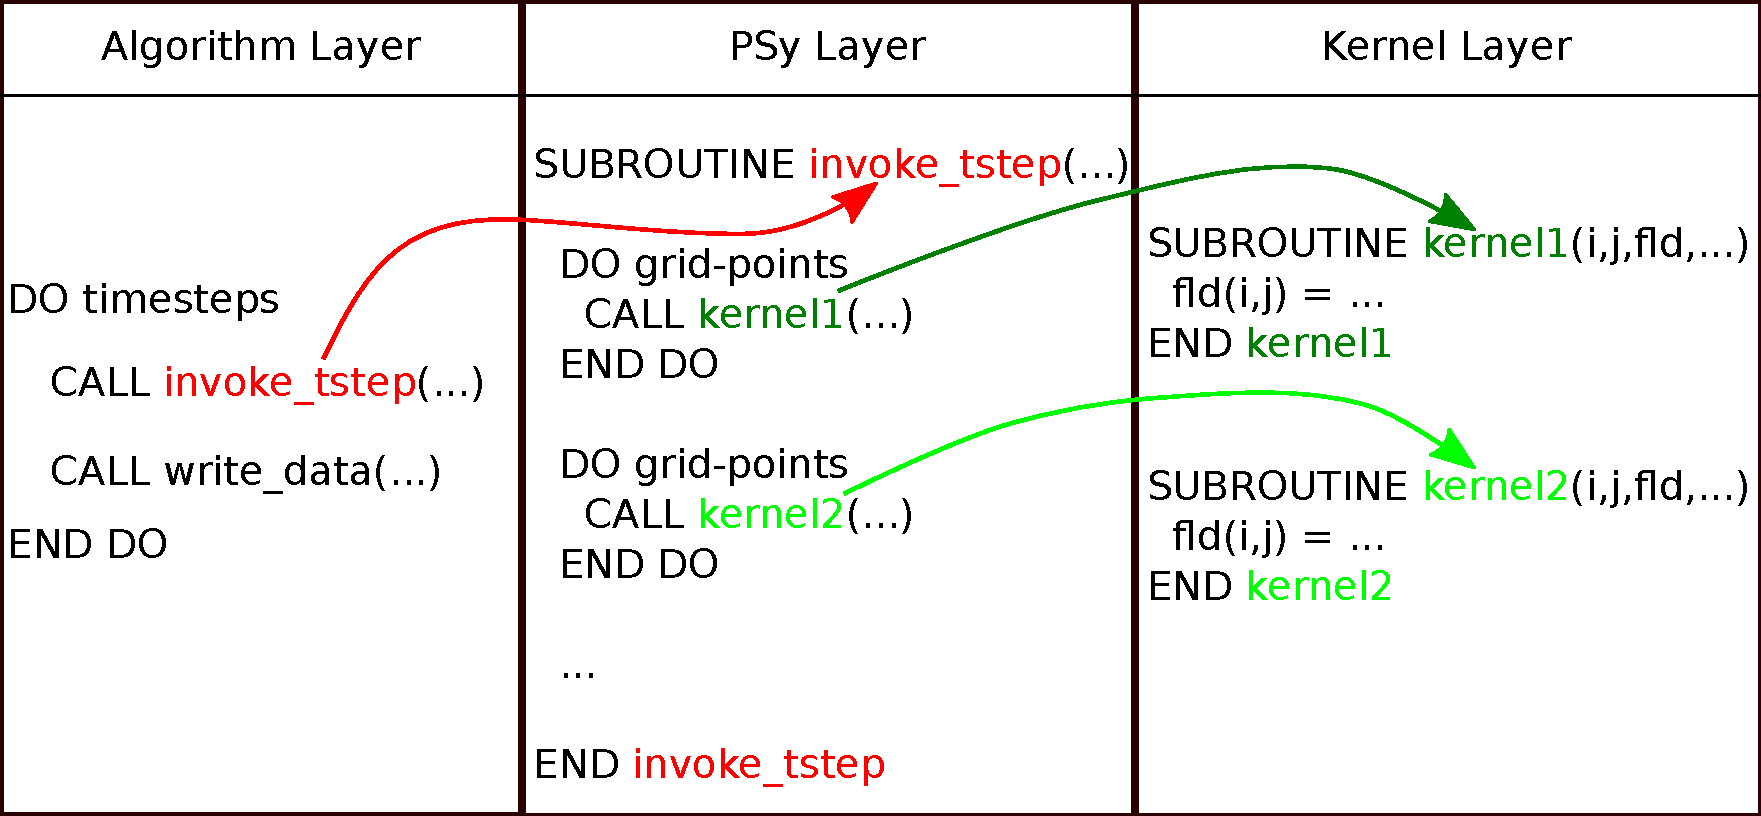
\includegraphics[width=85mm]{psykal_shallow}
\caption{A schematic of the vanilla \psykal version of the shallow code.}
\label{FIG_psykal_shallow_structure}
\end{figure}

As with any full oceanographic model, boundary conditions must be
applied at the edges of the model domain. In the case of Shallow we
have periodic boundary conditions in both the $x$ and $y$ dimensions.
These are simply implemented by having additional (`halo')
rows/columns at the edges of the domain and ensuring the data in them
is up-to-date before it is read. These rows/columns are updated by
copying data from the corresponding row/column on the opposite side of
the domain. In the current work, the lines of code to do these copies
is manually inserted in the PSy-layer routine as required.

{\bf Auto-generated BC code by reasoning about meta-data. But then,
  that brings us on to meta-data...}

%%%%%%%%%%%%%%%%%%%%%%%%%%%%%%%%%%%%%%%%%%%%%%%%%%%%%%%%%%%%%%%%%%%%
\section{Methodology(?)}

Our aim in this work is to achieve portable performance. Consequently,
we have performed tests with the hardware and compilers listed in
Table~\ref{TABLE_compilers}. Where a compiler is available on a given
piece of hardware, the version number used in this work is specified.
The Intel Haswell-based system (Xeon E5-1620 v2) has a clock speed of
3.7~GHz and 10~MB of last-level cache. The Intel Ivy Bridge-based
system (Xeon E5-2697) has a clock speed of 2.7~GHz and a last-level
cache of 30~MB. The CPU in the IBM Power-8 system is built around the
PowerPC xxx core with a clock speed of 4.1~GHz. The chip has xxx~MB of
last-level cache.

% An example of a floating table. Note that, for IEEE style tables, the 
% \caption command should come BEFORE the table. Table text will default to
% \footnotesize as IEEE normally uses this smaller font for tables.
% The \label must come after \caption as always.
%
\begin{table}[!t]
% increase table row spacing, adjust to taste
\renewcommand{\arraystretch}{1.3}
\caption{The matrix of compilers and CPUs used in this work. The use
  of a compiler on a given CPU is indicated by the specification of
  the version of the compiler in the relevent element. No entry
  indicates that a compiler was not available/used on that CPU.}
\label{TABLE_compilers}
\centering
\begin{tabular}{|l|c|c|c|c|}
\hline
                 & \multicolumn{4}{c|}{Compiler}             \\
\hline
                 & Gnu   & Intel       & Cray    & IBM     \\
\hline
Intel Haswell    & 4.8.2 & 14.0.0      &         &          \\
Intel Ivy Bridge & 4.9.1 & 14.0.1.106  & 8.3.3   &          \\
IBM Power 8      &       &             &         & 14.1     \\
\hline
\end{tabular}
\end{table}

In Table~\ref{TABLE_compiler_flags} we give the optimisation flags
used with each compiler. These flags are particularly important for
the \psykal versions of the code. The performance of the original
version of the code is much less sensitive to the compiler
options. This is because it consists of a single source file
containing effectively a single routine (excluding those for I/O).
 
\begin{table}[!t]
% increase table row spacing, adjust to taste
\renewcommand{\arraystretch}{1.3}
\caption{The compiler flags used in this work.}
\label{TABLE_compiler_flags}
\centering
\begin{tabular}{l|c}
\hline
Compiler  &  Flags \\
\hline
Gnu       & -Ofast -mtune=native -finline-limit=50000    \\
Intel     & -O3 -fast -fno-inline-factor    \\
Cray      & -O3 -O ipa5 -h wp               \\
IBM       & \bf{CHECK} -O5 -qinline=auto:level=10      \\
\hline
\end{tabular}
\end{table}

Before applying any code transformations, we benchmark the original
version of the code. We also benchmark the vanilla, unoptimised
version after it has been re-structured following the \psykal
approach. These two versions of the code effectively provide upper and
lower bounds, respectively, on the performance we expect to achieve.

{\bf Performance analysis as motivation for the code
  tranformations. More detail on each transformation.}

Beginning with the vanilla \psykal version, we then apply a series of
code transformations while obeying the \psykal separation of concerns,
{\it i.e.} optimisation is restricted to the middle, {PS}y layer and leaves
the kernel and algorithm layers unchanged. The aim of these
optimisations is to recover, as much as is possible, the structure and
thus performance of the original version of the code. The
transformations we have performed are as follows:
\begin{enumerate}

\item Pass explicit array bounds to middle layer (rather than using
  assumed-size array arguments)

\item Move kernel routines into same module as middle layer

\item Loop fusion

\item In-lined field-copy operation

\item Fused field-copy operation

\item Manually in-line kernel bodies into middle-layer code

\item Fully fuse first loop (only the outer loop of this loop nest was
  fused in the first pass)

\item Make the array/loop bounds explicitly constant for the
      duration of the time-stepping loop.
\end{enumerate}

We shall see that these transformations do not always result in improved
performance. Whether or not they do so depends both on the compiler
and the problem size. We also emphasise that the aim of these
optimisations is to recover, as far as is possible, the structure of
the original version of the code. It may well be that transforming the
code into some other structure would result in better performance on a
particular architecture. However, exploring this optimisation space is
beyond the scope of the present work.

We explore the extent to which performance depends upon the problem
size by using square domains of dimension 64, 128, 256, 512 and
1024. This range allows us to investigate what happens when cache is
exhausted as well as giving us some insight into the decisions that
different compilers make when optimising the code.

%%%%%%%%%%%%%%%%%%%%%%%%%%%%%%%%%%%%%%%%%%%%%%%%%%%%%%%%%%%%%%%%%%%%
\section{Results}

In Figure~\ref{FIG_orig_perf_summary} we plot the performance of the
original version of the shallow code for the range of compilers and
hardware considered here. This summary demonstrates the effect of the
larger last-level cache of the Intel Ivy Bridge system compared to
that of the Haswell system; note the significant drop in performance
in going from a problem size of $256^{2}$ to a problem size of
$512^{2}$ for the black and green bars. The performance of the Ivy
Bridge system with the Cray or Intel compiler (red and purple bars)
only drops to this level when the domain size is increased to
$1024^{2}$. At this point, the working set no longer fits within cache
and performance is dominated by the bandwidth to main memory, making
it relatively insensitive to the choice of compiler.

\begin{figure}[!t]
\centering
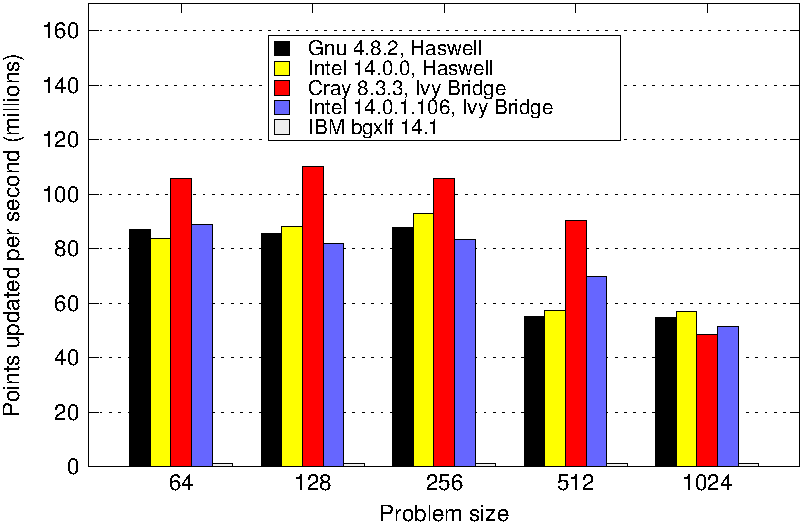
\includegraphics[width=2.8in]{orig_summary}
\caption{Summary of the performance of the original shallow code on 
the range of compilers and hardware under consideration.}
\label{FIG_orig_perf_summary}
\end{figure}

For this compiler-friendly form of the code, there is little
performance difference between the executables produced by the Gnu and
Intel compilers. However, the executable produced by the Cray compiler
generally performs significantly better. {\bf Why is this; can we work
out what it's doing that the others aren't?}

Note that the results for the Gnu compiler on Ivy Bridge show the same
drop-off (as problem size is increased) as those on the Haswell
system. This may be because Archer's login nodes seem to be running on
older hardware (E5-2650 with 20MB LLC) during the Archer upgrade. {\bf
  Need to re-run these cases once Archer is back up.}

Moving now the to the \psykal version of shallow,
Figure~\ref{FIG_best_psykal_perf_summary} plots the performance of the
fastest \psykal version for each of the compiler/CPU combinations. The
only significant difference between this and the plot of the
performance of the original version of the code in
Figure~\ref{FIG_orig_perf_summary} is that the difference between the
Gnu- and Intel-compiled executables is slightly more marked. This is
clarified in Figure~\ref{FIG_slowdown_summary} which plots the
percentage difference between the performance of the original and the
(best) \psykal versions of shallow for each compiler/CPU combination.
It is clear from this plot that the difference in the performance of
the Gnu- and Intel-compiled excutables on the Haswell system is due to
the Gnu compiler being unable to recover the performance achieved by
the original code. In contrast there is no such problem for the
Gnu-compiled executable on the Ivy Bridge system. We attribute this to
the more recent version of the compiler on the latter system (4.9.1 as
opposed to 4.8.2).

\begin{figure}[!t]
\centering
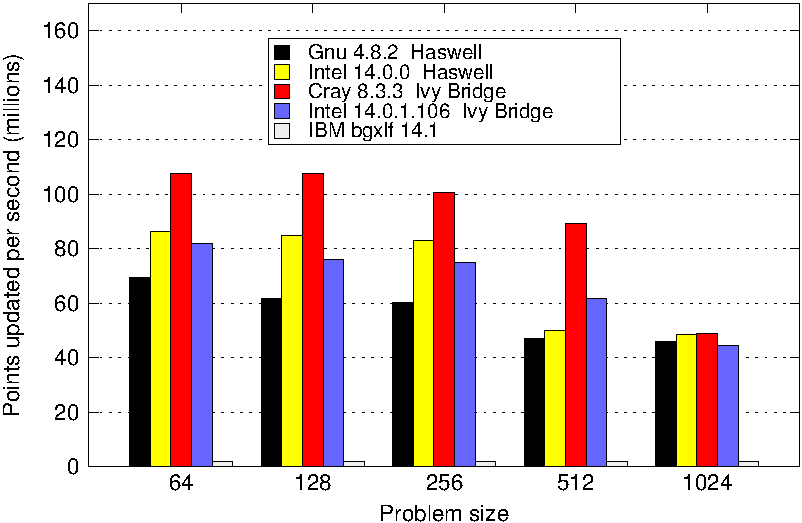
\includegraphics[width=7.5cm]{best_psykal_summary}
\caption{Summary of the best performance achieved by any \psykal 
version of shallow with each of the compilers and CPUs under 
consideration.}
\label{FIG_best_psykal_perf_summary}
\end{figure}

\begin{figure}[!t]
\centering
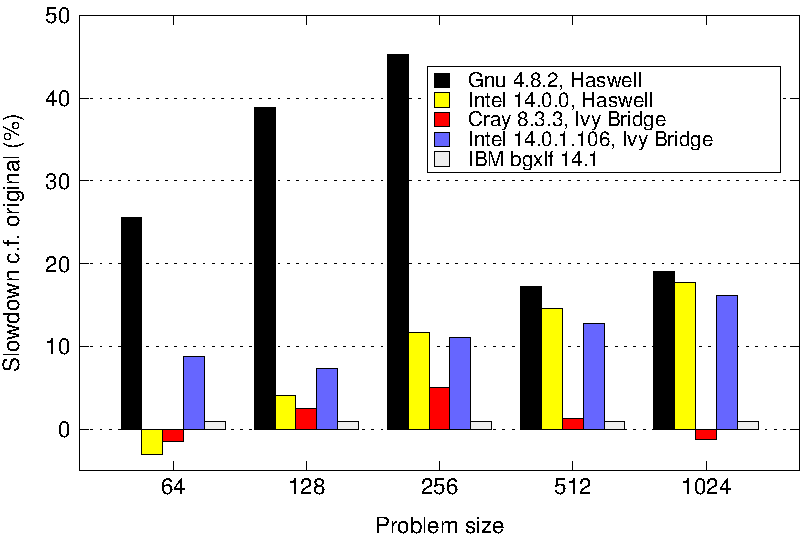
\includegraphics[width=2.8in]{slowdown_summary}
\caption{Comparison of the performance of the best \psykal
version with that of the original version of the code. A negative value 
indicates that the \psykal version is faster than the original.}
\label{FIG_slowdown_summary}
\end{figure}

In fact, for the Gnu and Cray compilers on the Ivy Bridge system, the
\psykal version of shallow is never more than 2\% slower than the
original and in some cases is faster.  This demonstrates that we can
reliably recover the performance of the original version of the code,
despite the significant restructuring required by the \psykal
approach.

Having show that, in general, we can recover and occasionally improve
upon the performance of the original version of shallow, the next
logical step is to examine the necessary code transformations.  We do
this for the $256^{2}$ case since this fits within cache on both the
Haswell and Ivy Bridge CPUs we are using here.
Table~\ref{TABLE_opt_breakdown} shows detailed timings for this case
after each transformation has been applied to the code. The same data
is visualised in Figure~\ref{FIG_opt_stages_256} where the performance
of the \psykal version for a given compiler/CPU is given relative to
the performance of the original with the same compiler/CPU. 

\begin{table*}[!t]
% increase table row spacing, adjust to taste
\renewcommand{\arraystretch}{1.3}
% if using array.sty, it might be a good idea to tweak the value of
% \extrarowheight as needed to properly center the text within the cells
\caption{The mean time-per-step (s) for the $256^2$ case after each 
code transformation.}
\label{TABLE_opt_breakdown}
\centering
\begin{tabular}{l|c|c|c|c|c|c}
\hline
Compiler:          &  Gnu  & Intel   & Gnu & Intel & Cray & IBM \\
\hline
CPU:               & \multicolumn{2}{c|}{Haswell} & \multicolumn{3}{c|}{Ivy Bridge} & Power8 \\
\hline
Original                               &  7.47E-04 & 7.06E-04 &	7.70E-04 & 7.77E-04 & 6.13E-04 &  1.17E-03  \\
Vanilla \psykal                        &  1.26E-02 & 8.64E-04 &	1.38E-02 & 9.82E-04 & 8.33E-04 &  7.87E-03  \\
Explicitly-sized arrays                &  1.26E-02 & 8.62E-04 &	1.38E-02 & 9.65E-04 & 6.96E-04 &  6.74E-03  \\
Kernels copied into module             &  1.10E-03 & 8.67E-04 &	9.42E-04 & 9.65E-04 & 7.10E-04 &  3.13E-03  \\
Loops fused                            &  1.09E-03 & 7.89E-04 &	9.07E-04 & 8.80E-04 & 7.35E-04 &  3.60E-03  \\
In-lined field-copy                    &  1.09E-03 & 7.90E-04 &	9.07E-04 & 8.73E-04 & 7.31E-04 &  3.62E-03  \\
Fused field-copy                       &  1.09E-03 & 9.25E-04 &	1.02E-03 & 1.04E-03 & 6.50E-04 &  4.11E-03  \\
In-line all kernels                    &  8.20E-04 & 7.14E-04 &	9.32E-04 & 8.52E-04 & 6.50E-04 &  1.07E-03  \\
Fully fuse 1st loop nest               &  8.10E-04 & 7.18E-04 &	7.76E-04 & 7.92E-04 & 6.23E-04 &  1.07E-03  \\
Explicit, constant array/loop bounds   &  8.05E-04 & 7.12E-04 &	7.81E-04 & 7.91E-04 & 6.13E-04 &  1.07E-03  \\
\hline
\parbox{2.5cm}{\%-slow-down of best {\it c.f.} original} & 7.8 & 0.8 & 0.8 & 1.8 & 0.03 & -9.0    \\
\hline
\end{tabular}
\end{table*}






















With the Gnu compiler (first and third clusters in
Figure~\ref{FIG_opt_stages_256}), the vanilla \psykal version of
shallow only achieves ~5-6\% of the performance of the
original. Simply copying the code for each of the kernel subroutines
into the module from which they are called has the most dramatic
effect on the performance of the compiled code; it now achieves almost
80\% of the performance of the original. The next most significant
transformation is that of (manually) in-lining the kernel code itself
into the bodies of the loops from which they are called. This gets the
\psykal version to within 8\% of the performance of the original.  The
dramatic performance improvement obtained from the first
transformation demonstrates that the Gnu compiler is unable to
optimise over separate files. Therefore, the fact that the
time-stepping loop in the \psykal version still retains a call to an
I/O routine and a call to the middle-layer, both of which are in
different files, is likely to account for this remaining performance
penalty of 8\%.

With the Intel compiler, the key transformations to recover
performance are different (second and fourth clusters in
Figure~\ref{FIG_opt_stages_256}).  Table~\ref{TABLE_opt_breakdown}
shows that even the vanilla \psykal version of shallow achieves some
80\% of the performance of the original version. Only two code
transformations were required to increase this to 100\%. The first of
these was the fusion of the computational loops. However, we found
that performance suffered (purple bar) when this was extended to
include the loop required for field copies at the end of a time-step
(Figure~\ref{FIG_time_smooth_code}). Further investigation of this
slow-down revealed that the compiler was unable to SIMD vectorise the
newly-fused loop after it had in-lined the body of the kernel called
from within it. Once this in-lining was done by hand (dark-blue bar),
the compiler was able to vectorise the loop and the performance of the
original version of shallow was recovered.

\begin{figure}[!t]
\centering
\includegraphics[width=95mm]{opt_stages_256}
\caption{The performance of the \psykal version of shallow for the
  $256^{2}$ domain at each stage of optimisation. Results are given as
  a percentage of the performance of the original code for each
  compiler/CPU combination. A figure greater than 100\% indicates that
  the \psykal version performs better than the original.}
\label{FIG_opt_stages_256}
\end{figure}

\begin{figure}
\begin{verbatim}
! Time smoothing
DO J=1,N+1
  DO I=1,M+1
    CALL time_smooth_code(i,j,ufld,unew,uold)
!    uold(i,j) = ufld(i,j) + alpha* &
!     (unew(i,j) - 2.*ufld(i,j) + uold(i,j))
  END DO
END DO

! Copy new fields into current fields
DO J=1,N+1
  DO I=1,M+1
    Ufld(I,J) = UNEW(I,J)
  END DO
END DO
\end{verbatim}
\caption{Example of the coding structure that required manual
  in-lining of the kernel body (as indicated by commented-out lines)
  to retrieve the performance of the original version of shallow with
  the Intel compiler.}
\label{FIG_time_smooth_code}
\end{figure}

The fifth cluster in Figure~\ref{FIG_opt_stages_256} shows the
evolution of the performance of the \psykal version of shallow with
the Cray compiler. Again, this has significant differences from the
behaviour seen with the Gnu and Intel compilers. As with the Intel
compiler, the performance of the Vanilla \psykal version is fairly
good at 74\% of that of the original. In contrast to the other
compilers consisdered so far, the first significant transformation is
simply to specify the bounds of the arrays being used within the
middle layer using module variables (as opposed to specifying them as
assumed size). This tells the compiler that all of the arrays used in
the middle layer have the same extent and also that all of the
computational loops are over almost all elements of these arrays. This
simple change gives a \psykal version that achieves 88\% of the
performance of the original.

Subsequent transformations actually harm performance until the
field-copy operation of Figure~\ref{FIG_time_smooth_code} is fused
with the preceeding loop. The resulting \psykal version now achieves
94\% of the original performance. Two further steps are required to
match the latter. First, the first loop nest has to be fully fused
(both inner and outer loops fused) and second, the array/loop bounds
are passed as an argument to the middle layer. This is done in order
to specify to the compiler that these bounds remain constant for the
duration of the time-stepping loop.

% An example of a double column floating figure using two subfigures.
% (The subfig.sty package must be loaded for this to work.)
% The subfigure \label commands are set within each subfloat command,
% and the \label for the overall figure must come after \caption.
% \hfil is used as a separator to get equal spacing.
% Watch out that the combined width of all the subfigures on a 
% line do not exceed the text width or a line break will occur.

%
%\begin{figure*}[!t]
%\centering
%\subfloat[Case I]{\includegraphics[width=2.5in]{box}%
%\label{fig_first_case}}
%\hfil
%\subfloat[Case II]{\includegraphics[width=2.5in]{box}%
%\label{fig_second_case}}
%\caption{Simulation results.}
%\label{fig_sim}
%\end{figure*}
%
% Note that often IEEE papers with subfigures do not employ subfigure
% captions (using the optional argument to \subfloat[]), but instead will
% reference/describe all of them (a), (b), etc., within the main caption.




% Note that IEEE does not put floats in the very first column - or typically
% anywhere on the first page for that matter. Also, in-text middle ("here")
% positioning is not used. Most IEEE journals use top floats exclusively.
% Note that, LaTeX2e, unlike IEEE journals, places footnotes above bottom
% floats. This can be corrected via the \fnbelowfloat command of the
% stfloats package.



\section{Conclusions}

We have investigated the application of the \psykal separation of
concerns approach to the domain of finite-difference ocean
models. This approach enables the computational science (performance)
related aspects of a computer model to be kept separate from the
natural (oceanographic) science aspects. In this work we have shown
that the \psykal approach has the potential to improve performance and
to improve code structure/maintainability.

The application of code transformations to the middle/PSy layer is key
to the performance of the \psykal version of a code.




% use section* for acknowledgement
\section*{Acknowledgments}


This work made use of the ARCHER UK National Supercomputing Service
(\url{http://www.archer.ac.uk}).

% http://www.ctan.org/tex-archive/biblio/bibtex/contrib/doc/
% The IEEEtran BibTeX style support page is at:
% http://www.michaelshell.org/tex/ieeetran/bibtex/
\bibliographystyle{IEEEtran}
% argument is your BibTeX string definitions and bibliography database(s)
\bibliography{IEEEabrv,shallow_perf}
%

% biography section
% 
% If you have an EPS/PDF photo (graphicx package needed) extra braces are
% needed around the contents of the optional argument to biography to prevent
% the LaTeX parser from getting confused when it sees the complicated
% \includegraphics command within an optional argument. (You could create
% your own custom macro containing the \includegraphics command to make things
% simpler here.)
%\begin{IEEEbiography}[{\includegraphics[width=1in,height=1.25in,clip,keepaspectratio]{mshell}}]{Michael Shell}
% or if you just want to reserve a space for a photo:

\begin{IEEEbiographynophoto}{A.~R.~Porter}
Biography text here.
\end{IEEEbiographynophoto}

% if you will not have a photo at all:
\begin{IEEEbiographynophoto}{R.~Ford}
Biography text here.
\end{IEEEbiographynophoto}

% insert where needed to balance the two columns on the last page with
% biographies
%\newpage

\begin{IEEEbiographynophoto}{G.~Riley}
Biography text here.
\end{IEEEbiographynophoto}

% You can push biographies down or up by placing
% a \vfill before or after them. The appropriate
% use of \vfill depends on what kind of text is
% on the last page and whether or not the columns
% are being equalized.

%\vfill

% Can be used to pull up biographies so that the bottom of the last one
% is flush with the other column.
%\enlargethispage{-5in}


% that's all folks
\end{document}


